\documentclass[11pt]{article}
\usepackage[utf8]{inputenc}
\usepackage[T1]{fontenc}
\usepackage{lmodern}
\usepackage{amsmath,amssymb,amsthm}
\usepackage{microtype}
\microtypesetup{expansion=false}
\usepackage{graphicx}
\usepackage{xcolor}
\usepackage[margin=1in]{geometry}
\usepackage{datetime2}
\DTMsetup{showzone=false}
\usepackage{enumitem}
\usepackage{booktabs}
\usepackage{caption}
\captionsetup{font=small,labelfont=bf}
\usepackage[colorlinks=true,linkcolor=blue!55!black,urlcolor=teal!60!black,citecolor=purple!55!black]{hyperref}

\DeclareMathOperator{\tr}{tr}
\DeclareMathOperator{\Cov}{Cov}
\DeclareMathOperator{\Var}{Var}
\DeclareMathOperator{\df}{df}
\newcommand{\E}{\mathbb{E}}
\newcommand{\Rb}{\mathbb{R}}
\newcommand{\yhat}{\hat y}

\theoremstyle{definition}
\newtheorem{example}{Example}
\newtheorem{exercise}{Exercise}
\theoremstyle{plain}
\newtheorem{lemma}{Lemma}
\newtheorem{theorem}{Theorem}

\newcommand{\keyidea}[1]{\par\smallskip\noindent%
\fcolorbox{blue!45!black}{blue!5}{\parbox{\dimexpr\linewidth-2\fboxsep-2\fboxrule}%
{\small\textbf{Key idea.}\ #1}}\par\smallskip}

\setlength{\parskip}{0.35em}
\setlength{\parindent}{0pt}

\begin{document}

\begin{center}
{\LARGE\bfseries Effective Degrees of Freedom}\\[3pt]
{\large from covariance penalties to the Jacobian trace}\\[10pt]
{\small An expository companion to the LPS Tier-0 specification, gate E0.2}\\[8pt]
{\footnotesize Source: \nolinkurl{/Users/pgajer/current_projects/geosmooth/project_briefs/effective_degrees_of_freedom_note_2026-06-10.tex}}\\[2pt]
{\footnotesize Compiled \DTMnow\ ET}
\end{center}

\vspace{0.5em}
\hrule
\vspace{1em}

This note expands one line of the E0.2 gate, the claim that
$\df = \tr S = \sum_i \partial \yhat_i/\partial y_i$, into a short self-contained
tour of what \emph{effective degrees of freedom} means, why it is defined the way
it is, and why a true mathematical identity can still be a useful software test.
Everything is illustrated with a simple example and a figure, and there are
exercises (with answers) at the end.

\tableofcontents
\vspace{1em}
\hrule
\vspace{1em}

%==================================================================
\section{The puzzle: how many parameters does a smoother use?}

In ordinary least squares with $p$ predictors, the fitted values are a linear
projection of the data, $\yhat = Hy$, where $H$ is the ``hat matrix.'' Its trace
counts the parameters, $\tr H = p$, and we call $p$ the model's
\emph{degrees of freedom}: it is how many directions in $y$ the fit is free to
chase. Residual degrees of freedom are $n-p$, the denominator in the variance
estimate.

Now fit a smoothing spline, a $k$-nearest-neighbour average, a local polynomial,
the lasso, or a regression tree. There is no obvious ``$p$.'' Yet software
routinely reports things like ``spline with \texttt{df}~$=7.3$.'' What is that
number, and in what sense is it the right generalisation of ``number of
parameters''?

We want a definition of $\df$ that satisfies three things at once: it
\emph{(a)} reduces to $p$ for OLS; \emph{(b)} measures something operational ---
how much the procedure overfits; and \emph{(c)} is computable for \emph{any}
fitting rule, linear or not. Remarkably, one quantity does all three, and it
wears three equivalent faces --- a covariance, an average derivative, and a
matrix trace (Figure~\ref{fig:threelenses}, later). The rest of the note builds
it.

%==================================================================
\section{Optimism: why training error lies}

Write the data as signal plus noise, $y_i = \mu_i + \varepsilon_i$, with the
$\varepsilon_i$ uncorrelated, mean $0$, variance $\sigma^2$. A fitting procedure
maps the data to fitted values, $\yhat = m(y)$. Two error measures matter:

\begin{itemize}[nosep,leftmargin=1.4em]
\item \emph{training (apparent) error} $\ \mathrm{err}=\tfrac1n\sum_i (y_i-\yhat_i)^2$,
the error on the very data used to fit;
\item \emph{test (prediction) error} $\ \mathrm{Err}=\tfrac1n\sum_i \E(y_i^\ast-\yhat_i)^2$,
where $y_i^\ast=\mu_i+\varepsilon_i^\ast$ is a fresh independent observation at the
same $x_i$ and $\yhat$ is held fixed from the original data.
\end{itemize}

Training error is optimistic: the fit has already seen $y$, so it explains part
of the noise. The gap is exactly a covariance.

\begin{theorem}[Optimism]\label{thm:optimism}
$\displaystyle \E[\mathrm{Err}] - \E[\mathrm{err}] \;=\; \frac{2}{n}\sum_{i=1}^n \Cov(\yhat_i, y_i).$
\end{theorem}

\begin{proof}
Work point by point. Because $y_i^\ast$ is an independent copy of $y_i$, it has the
same first two moments, and $y_i^\ast$ is independent of $\yhat_i$ (which is a
function of the original $y$). Expanding the squares,
\[
\E[(y_i^\ast-\yhat_i)^2]-\E[(y_i-\yhat_i)^2]
= \underbrace{\big(\E[y_i^{\ast2}]-\E[y_i^2]\big)}_{=\,0}
- 2\big(\E[y_i^\ast \yhat_i]-\E[y_i \yhat_i]\big).
\]
Independence gives $\E[y_i^\ast \yhat_i]=\E[y_i^\ast]\,\E[\yhat_i]=\mu_i\E[\yhat_i]$,
while $\E[y_i \yhat_i]=\Cov(y_i,\yhat_i)+\mu_i\E[\yhat_i]$. The difference is
$-\Cov(y_i,\yhat_i)$, so the bracket equals $2\Cov(\yhat_i,y_i)$. Average over $i$.
\end{proof}

So $\sum_i \Cov(\yhat_i,y_i)$ \emph{is} the amount of overfitting --- how much the
fit's values move \emph{with} their own observations. Normalising by the noise
level turns it into a pure count.

\keyidea{Efron's definition of effective degrees of freedom is
$\displaystyle \df \;=\; \frac{1}{\sigma^2}\sum_{i=1}^n \Cov(\yhat_i, y_i).$
It is the covariance penalty that corrects training error:
$\E[\mathrm{Err}]\approx \E[\mathrm{err}] + \tfrac{2\sigma^2}{n}\df$ (Mallows' $C_p$).}

\begin{example}[OLS recovers $p$]
For $\yhat=Hy$, $\Cov(\yhat_i,y_i)=\Cov\big(\sum_j H_{ij}y_j,\,y_i\big)=H_{ii}\sigma^2$,
since distinct observations are uncorrelated. Hence
$\df=\sigma^{-2}\sum_i H_{ii}\sigma^2=\tr H=p$. A straight-line fit
($p=2$: intercept and slope) has $\df=2$ and optimism $4\sigma^2/n$.
\end{example}

Figure~\ref{fig:optimism} shows the mechanism directly: as model complexity grows,
training error falls monotonically while test error turns up, and the gap between
them widens in exact proportion to $\df$.

\begin{figure}[h]
\centering
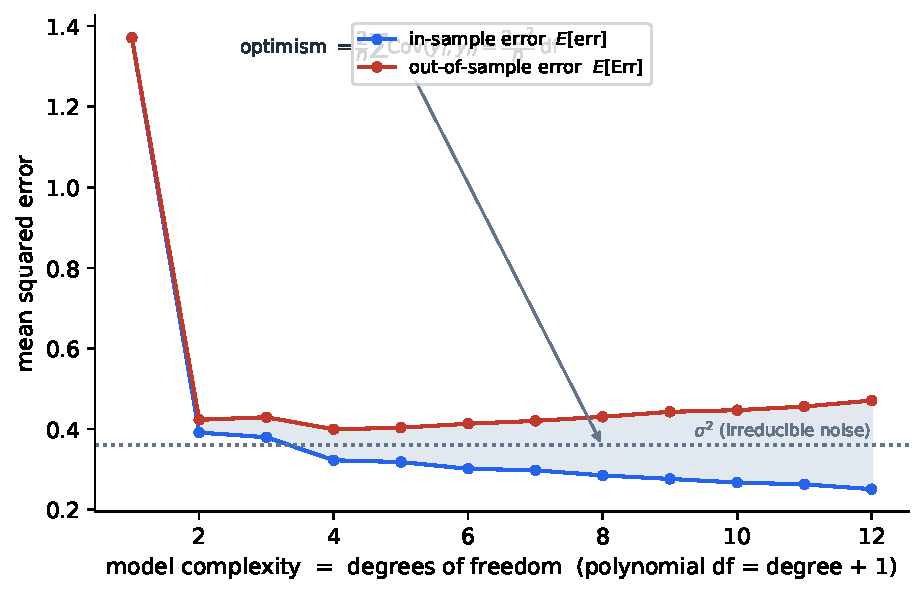
\includegraphics[width=0.82\linewidth]{figures_edf/fig_optimism.pdf}
\caption{Polynomials of increasing degree fit to noisy data (averaged over $500$
replications). In-sample error keeps dropping, but out-of-sample error is
U-shaped; the shaded gap is the optimism $\tfrac{2}{n}\sum_i\Cov(\yhat_i,y_i)
=\tfrac{2\sigma^2}{n}\df$. Degrees of freedom is precisely the knob that sets how
far training error understates the truth.}
\label{fig:optimism}
\end{figure}

%==================================================================
\section{The smoother matrix and self-sensitivity}

A \emph{linear smoother} writes the fit as $\yhat = Sy$ for a matrix $S$ that
depends on the design $X$ (positions, bandwidth, degree, kernel) but \emph{not} on
$y$. The diagonal entry
\[
S_{ii} \;=\; \frac{\partial \yhat_i}{\partial y_i}
\]
is the \emph{self-sensitivity} (or leverage) of point $i$: nudge the single
observation $y_i$ and watch how much its own fitted value follows. A fit that
chases the data has $S_{ii}\approx 1$; a heavy smoother that averages many points
has $S_{ii}\approx 0$ (Figure~\ref{fig:selfsens}).

\begin{figure}[h]
\centering
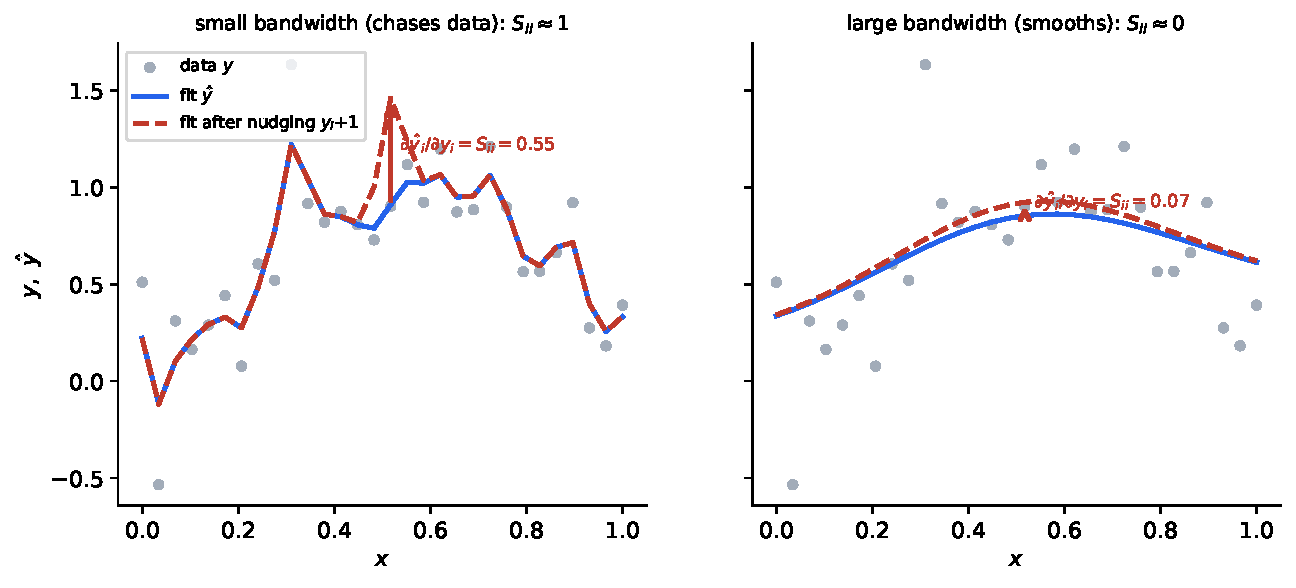
\includegraphics[width=0.95\linewidth]{figures_edf/fig_selfsens.pdf}
\caption{Self-sensitivity made visible. The same point $y_i$ is nudged up by $1$
(solid $\to$ dashed). With a small bandwidth (left) the fit tracks the point
almost one-for-one, $S_{ii}\approx1$; with a large bandwidth (right) the fit
barely moves, $S_{ii}\approx0$. The vertical red arrow is the realised change
$\yhat_i$, which equals $S_{ii}$ because the nudge has size $1$.}
\label{fig:selfsens}
\end{figure}

The covariance definition collapses to a trace here, and --- worth noting --- with
no distributional assumption beyond uncorrelated, equal-variance errors:
\[
\Cov(\yhat_i,y_i)=\Cov\Big(\textstyle\sum_j S_{ij}y_j,\;y_i\Big)=S_{ii}\,\sigma^2
\quad\Longrightarrow\quad
\df=\sum_i S_{ii}=\tr S.
\]

\keyidea{For any linear smoother $\yhat=Sy$, $\ \df=\tr S$, the sum of the
self-sensitivities. This is the form most often quoted for splines and kernel
smoothers.}

\begin{figure}[h]
\centering
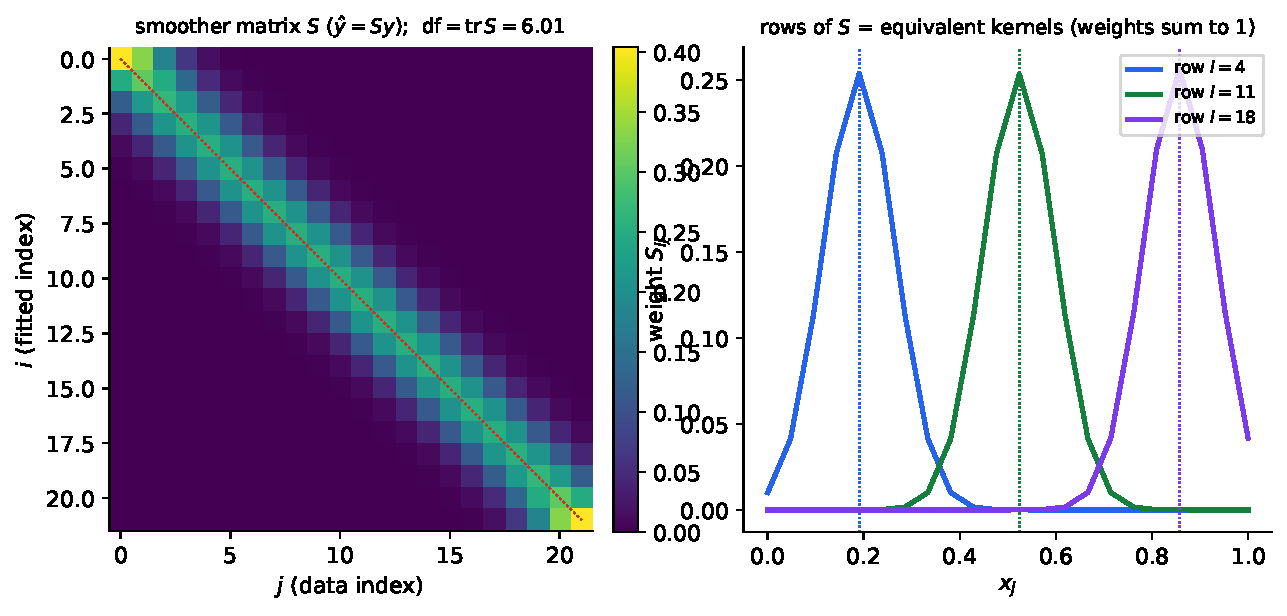
\includegraphics[width=0.95\linewidth]{figures_edf/fig_smatrix.pdf}
\caption{Left: the smoother matrix $S$ of a kernel smoother; the dotted line is the
diagonal, and $\df=\tr S$ sums those diagonal entries. Right: individual rows of
$S$ are the ``equivalent kernels'' --- the weights each fitted value places on the
data (they sum to $1$).}
\label{fig:smatrix}
\end{figure}

\begin{example}[$k$-nearest-neighbour average]
If $\yhat_i$ is the average of the $k$ observations nearest $x_i$ (counting point
$i$ itself), then the weight on $y_i$ is $1/k$, so $S_{ii}=1/k$ and
$\df=\tr S = n/k$. With $k=1$ the smoother interpolates, $\df=n$; with $k=n$ it is
the global mean, $\df=1$. Degrees of freedom slides continuously between these as
$k$ changes.
\end{example}

%==================================================================
\section{Stein's lemma}

To extend ``$\df=\tr S$'' to \emph{nonlinear} fits we need a bridge from the
covariance form to a derivative. That bridge is Stein's lemma, a small but
powerful consequence of integration by parts against the Gaussian density.

\begin{lemma}[Stein, 1981]\label{lem:stein}
If $Z\sim N(\mu,\sigma^2)$ and $g$ is absolutely continuous with $\E|g'(Z)|<\infty$,
then $\ \Cov\big(Z,g(Z)\big)=\sigma^2\,\E[g'(Z)].$
\end{lemma}

\begin{proof}
The normal density $\varphi$ satisfies $\varphi'(z)=-\tfrac{z-\mu}{\sigma^2}\varphi(z)$,
i.e. $(z-\mu)\varphi(z)=-\sigma^2\varphi'(z)$ (Figure~\ref{fig:stein}, left). Then
\[
\E[(Z-\mu)g(Z)] = \int (z-\mu)g(z)\varphi(z)\,dz
= -\sigma^2\!\int g(z)\varphi'(z)\,dz
= \sigma^2\!\int g'(z)\varphi(z)\,dz = \sigma^2\E[g'(Z)],
\]
integrating by parts (the boundary terms vanish under the stated conditions).
\end{proof}

The multivariate version, applied coordinatewise: if $y\sim N(\mu,\sigma^2 I_n)$ and
$h:\Rb^n\to\Rb$ is weakly differentiable with integrable partials, then
$\Cov(y_i,h(y))=\sigma^2\,\E[\partial h/\partial y_i]$.

\begin{figure}[h]
\centering
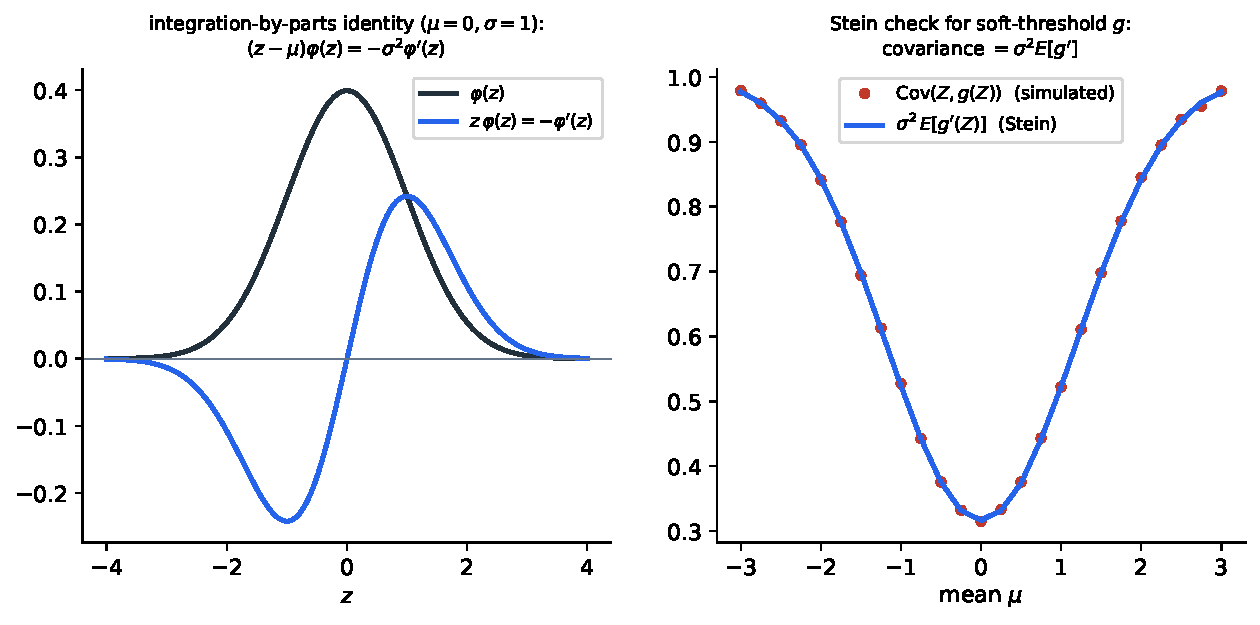
\includegraphics[width=0.95\linewidth]{figures_edf/fig_stein.pdf}
\caption{Left: the integration-by-parts identity behind Stein's lemma,
$(z-\mu)\varphi(z)=-\sigma^2\varphi'(z)$. Right: a numerical check for the
soft-threshold $g(z)=\mathrm{sign}(z)(|z|-\lambda)_+$, whose derivative is the
indicator $\mathbf 1\{|z|>\lambda\}$: the simulated covariance matches
$\sigma^2\E[g']$ across the mean $\mu$.}
\label{fig:stein}
\end{figure}

\begin{example}[two quick checks]
For $g(z)=z$: $\Cov(Z,Z)=\sigma^2$ and $\sigma^2\E[g']=\sigma^2$. For $g(z)=z^2$ with
$Z\sim N(\mu,\sigma^2)$: $\Cov(Z,Z^2)=2\mu\sigma^2$, and
$\sigma^2\E[2Z]=2\mu\sigma^2$. The soft-threshold $g$ of
Figure~\ref{fig:stein} has $g'=\mathbf 1\{|z|>\lambda\}$, so
$\Cov(Z,g(Z))=\sigma^2\,\Pr(|Z|>\lambda)$ --- a preview of the lasso.
\end{example}

%==================================================================
\section{Putting it together: covariance $=$ expected divergence}

Apply the multivariate lemma with $h(y)=\yhat_i=m_i(y)$, the $i$-th fitted value
seen as a function of the whole data vector:
\[
\Cov(\yhat_i,y_i)=\sigma^2\,\E\!\Big[\frac{\partial \yhat_i}{\partial y_i}\Big].
\]
Summing over $i$ and dividing by $\sigma^2$,
\[
\boxed{\ \df \;=\; \frac{1}{\sigma^2}\sum_i \Cov(\yhat_i,y_i)
\;=\; \E\Big[\sum_i \frac{\partial \yhat_i}{\partial y_i}\Big]
\;=\; \E\big[\tr J(y)\big]\ }
\]
where $J(y)=\partial\yhat/\partial y$ is the Jacobian of the fitting map, with
entries $J_{ij}=\partial\yhat_i/\partial y_j$. The sum of its diagonal,
$\sum_i \partial\yhat_i/\partial y_i$, is the \emph{divergence} of $y\mapsto\yhat$.
So degrees of freedom is the expected divergence of the fit --- ``Stein's unbiased
degrees of freedom,'' the quantity inside the SURE risk estimate.

\begin{figure}[h]
\centering
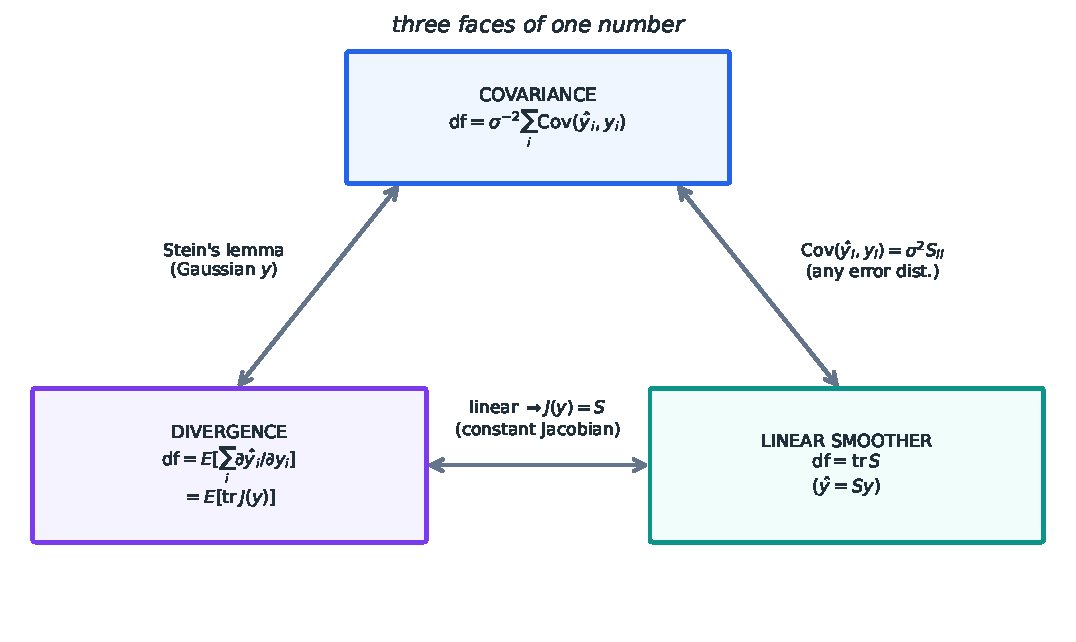
\includegraphics[width=0.72\linewidth]{figures_edf/fig_threelenses.pdf}
\caption{One number, three faces. Efron's covariance form and the
divergence/Jacobian-trace form are linked by Stein's lemma (and so require
Gaussian $y$); both collapse to $\tr S$ for a linear smoother, where the Jacobian
$J(y)=S$ is constant. The covariance-to-$\tr S$ edge needs only uncorrelated,
equal-variance errors --- no normality.}
\label{fig:threelenses}
\end{figure}

Two remarks pin down the logical status. \emph{First}, for a linear smoother
$J(y)=S$ for every $y$, so the expectation is vacuous and $\df=\tr S$ exactly --- no
Gaussianity needed. \emph{Second}, for a general fit the Jacobian depends on $y$,
and the \emph{sample} divergence $\tr J(y)$ evaluated at the observed data is an
\emph{unbiased estimate} of $\df$. When no formula exists, one estimates it by
finite differences or random perturbations of $y$ (Ye's ``generalized degrees of
freedom''). This sample divergence is exactly what the E0.2 bump-trace computes.

%==================================================================
\section{A gallery of degrees of freedom}

\begin{itemize}[leftmargin=1.4em]
\item \textbf{OLS:} $\df=\tr H=p$ (an integer; the anchor case).
\item \textbf{Ridge regression:} $\df(\lambda)=\sum_j d_j^2/(d_j^2+\lambda)$, where
$d_j$ are the singular values of the design. It decreases smoothly from $p$ (at
$\lambda=0$) to $0$ (as $\lambda\to\infty$); see Figure~\ref{fig:ridge}. Degrees of
freedom is generally \emph{not an integer}.
\item \textbf{Smoothing spline:} $\df=\tr S(\lambda)$; practitioners often choose
and report $\df$ rather than the opaque penalty $\lambda$.
\item \textbf{$k$-NN:} $\df=n/k$.
\item \textbf{Lasso / soft-threshold:} $\df=\E[\,\#\{\text{nonzero coefficients}\}\,]$
(Zou--Hastie--Tibshirani). In the orthonormal case this follows from the
soft-threshold derivative of the previous section: each coordinate contributes
$\mathbf 1\{|z_j|>\lambda\}$. Degrees of freedom literally counts the variables the
procedure \emph{effectively selects} --- but as an expectation that already accounts
for the adaptivity of the selection.
\item \textbf{Interpolation:} $\yhat=y$ gives $S=I$, $\df=\tr I=n$ --- maximal
complexity, zero training error, and (Exercise~6) useless predictions.
\end{itemize}

\begin{figure}[h]
\centering
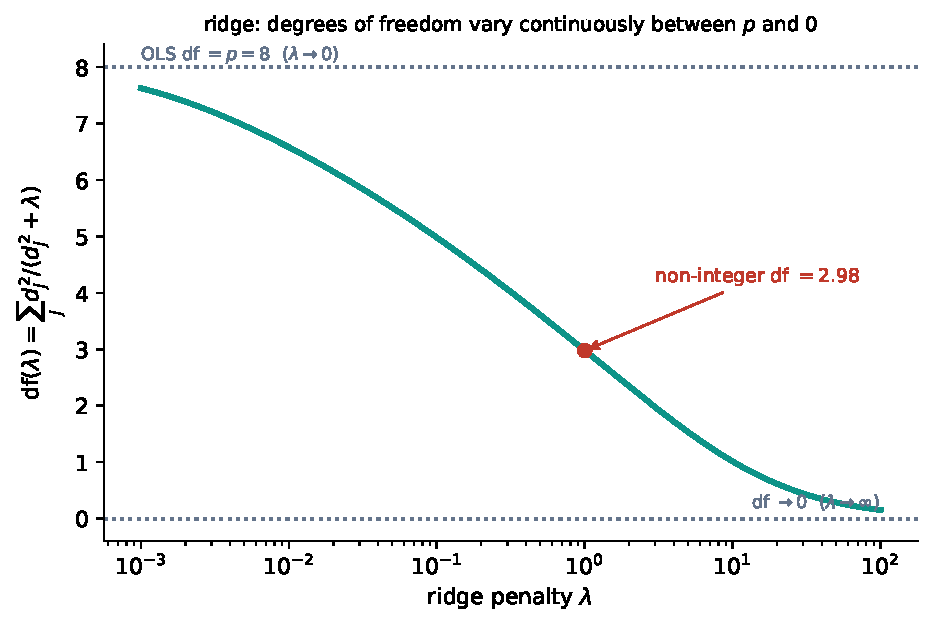
\includegraphics[width=0.78\linewidth]{figures_edf/fig_ridge.pdf}
\caption{Ridge degrees of freedom $\df(\lambda)=\sum_j d_j^2/(d_j^2+\lambda)$ vary
continuously between the parameter count $p$ and $0$. ``Effective'' degrees of
freedom is generally a real number, not a count.}
\label{fig:ridge}
\end{figure}

\keyidea{``This definition applies to any fitter, linear or not.''\ \ The
self-sensitivity / divergence definition needs no parameter count, no linear
structure, and no integer --- only that the fit responds to perturbing the data. So
it assigns a meaningful, comparable $\df$ to splines, $k$-NN, the lasso, trees, even
neural nets. The classical ``$\df=$ number of parameters'' is the special case where
$\yhat=Hy$ and $\tr H=p$ happens to be an integer.}

%==================================================================
\section{Back to the test: E0.2 as software falsification}

For the \emph{ideal} linear operator $S$, the equality
$\df=\tr S=\sum_i\partial\yhat_i/\partial y_i$ is a theorem --- it cannot be
empirically false. So what does E0.2 test? Not the theorem; the \emph{code}. There
are two objects: the linear-algebra ideal $S$, and the compiled function
\texttt{fit.lps} that may or may not actually realise it. The test computes the two
sides by two \emph{independent} routes and checks they agree:

\begin{itemize}[nosep,leftmargin=1.4em]
\item \textbf{Route A} --- reconstruct $S$ column by column from
$S_{\cdot j}=\texttt{fit}(e_j)$ (feed unit-basis responses), then take $\tr S$.
\item \textbf{Route B} --- finite-difference the self-sensitivities around a
\emph{generic} random $y$: bump $y_i$ by $\varepsilon=1$ and sum
$\texttt{fit}(y+e_i)_i-\texttt{fit}(y)_i$.
\end{itemize}

If the implemented map is genuinely linear and $y$-independent, the two routes
agree exactly (the theorem), and the step $\varepsilon=1$ is exact because for a
linear map the secant equals the derivative with no truncation error. If instead
there is any hidden $y$-dependence, the Jacobian varies with the operating point,
the two routes probe different points ($\{e_j\}$ near the origin versus a generic
$y$), and they \emph{disagree} (Figure~\ref{fig:tworoute}).

\begin{figure}[h]
\centering
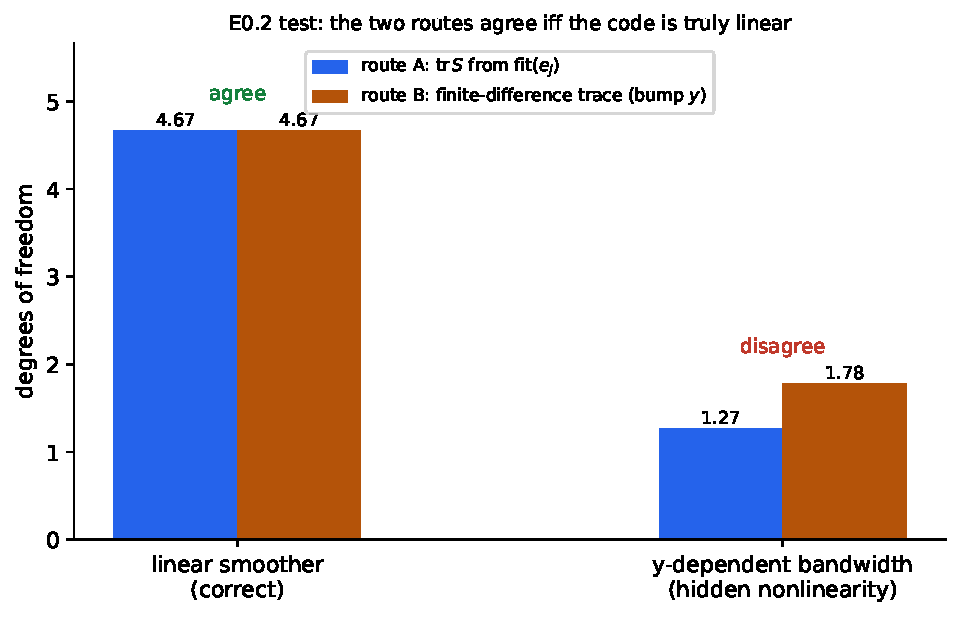
\includegraphics[width=0.74\linewidth]{figures_edf/fig_tworoute.pdf}
\caption{The two routes on a genuine linear smoother (left) agree to rounding; on a
``smoother'' whose bandwidth secretly depends on $y$ (right) they disagree, because
its Jacobian is not constant. The gap is a falsification signal: the code is not the
linear operator it claims to be.}
\label{fig:tworoute}
\end{figure}

Real culprits for such hidden $y$-dependence: a bandwidth chosen from the spread of
$y$; a ridge that activates only when a $y$-dependent condition number exceeds a
cap; probability clipping; or an ``unstable-action'' fallback keyed to the
magnitudes of $y$. Any of these would silently break every downstream variance, df,
and CV-shortcut formula that assumes a fixed $S$.

\keyidea{The theorem is the \emph{oracle}; the test is a \emph{falsification} of the
software. A correct implementation is forced to satisfy a relationship a buggy
(nonlinear, $y$-dependent, or mis-accounted) one will violate --- which is why a
``trivially true'' identity makes a sharp unit test.}

%==================================================================
\section*{Exercises}
\addcontentsline{toc}{section}{Exercises}

\begin{exercise}
A $k$-NN running-mean smoother sets $\yhat_i$ to the average of the $k$
observations nearest $x_i$, counting $i$ itself. Show $S_{ii}=1/k$ and $\df=n/k$.
What are the two extremes $k=1$ and $k=n$?
\end{exercise}

\begin{exercise}
On $n=6$ ordered points, the width-$3$ moving average sets
$\yhat_i=(y_{i-1}+y_i+y_{i+1})/3$ for interior $i$, and at the ends
$\yhat_1=(y_1+y_2)/2$, $\yhat_6=(y_5+y_6)/2$. Compute $\tr S$.
\end{exercise}

\begin{exercise}
Let $Z\sim N(0,1)$ and $g(z)=z^3$. Compute $\Cov(Z,Z^3)$ and $\sigma^2\E[g'(Z)]$
directly and check Stein's lemma.
\end{exercise}

\begin{exercise}
For ridge, $\df(\lambda)=\sum_j d_j^2/(d_j^2+\lambda)$. Show $\df(\lambda)$ is
strictly decreasing in $\lambda$, with limits $p$ and $0$.
\end{exercise}

\begin{exercise}
In an orthonormal design the lasso gives $\hat\beta_j=\mathrm{sign}(z_j)(|z_j|-\lambda)_+$
with $z=X^\top y$. Using the divergence definition, show
$\df=\E[\,\#\{j:|z_j|>\lambda\}\,]$, the expected number of selected variables.
\end{exercise}

\begin{exercise}
A fit interpolates the data, $\yhat=y$. What is $\df$? Using
Theorem~\ref{thm:optimism}, what is the test error, and why is a zero training
error misleading?
\end{exercise}

\begin{exercise}
In the E0.2 test, suppose route A ($\tr S$ from $\texttt{fit}(e_j)$) and route B
(finite-difference trace around a random $y$) disagree well beyond rounding. What
does this tell you about the implementation, and give one concrete code bug that
would cause it?
\end{exercise}

%==================================================================
\section*{Answers}
\addcontentsline{toc}{section}{Answers}

\textbf{1.} $\yhat_i=\frac1k\sum_{j\in N_i}y_j$ with $i\in N_i$, so the coefficient
on $y_i$ is $1/k$, i.e. $S_{ii}=1/k$. Then $\df=\tr S=\sum_{i=1}^n \frac1k=n/k$.
$k=1$: $\yhat=y$, $\df=n$ (interpolation); $k=n$: global mean, $\df=1$.

\textbf{2.} Interior indices $i=2,3,4,5$ each contribute $S_{ii}=1/3$; the two ends
contribute $S_{11}=S_{66}=1/2$. So $\tr S = 4\cdot\frac13 + 2\cdot\frac12
= \frac43 + 1 = \frac73 \approx 2.33$. (A width-$3$ average ``spends'' about $2.3$
parameters on $6$ points.)

\textbf{3.} $\Cov(Z,Z^3)=\E[Z^4]-\E[Z]\E[Z^3]=3-0=3$. And
$\sigma^2\E[g'(Z)]=1\cdot\E[3Z^2]=3\E[Z^2]=3$. They agree.

\textbf{4.} Each term $t_j(\lambda)=d_j^2/(d_j^2+\lambda)$ has
$t_j'(\lambda)=-d_j^2/(d_j^2+\lambda)^2<0$, so $\df$ is strictly decreasing. As
$\lambda\to0$, $t_j\to1$ and $\df\to p$; as $\lambda\to\infty$, $t_j\to0$ and
$\df\to0$. Thus $\df$ ranges continuously over $(0,p)$.

\textbf{5.} With an orthonormal design the coordinates decouple and
$\partial\hat\beta_j/\partial z_j=\mathbf 1\{|z_j|>\lambda\}$ (the soft-threshold is
flat inside $[-\lambda,\lambda]$ and unit-slope outside). The fitted values inherit
the same diagonal Jacobian, so
$\sum_i\partial\yhat_i/\partial y_i=\#\{j:|z_j|>\lambda\}$, and taking expectations,
$\df=\E[\#\{|z_j|>\lambda\}]$ --- the expected size of the active set. (Note it is an
expectation: the realised active-set size is the \emph{unbiased estimate} of $\df$.)

\textbf{6.} $S=I$, so $\df=\tr I=n$. Every $\partial\yhat_i/\partial y_i=1$.
Training error is $0$, but by Theorem~\ref{thm:optimism} the optimism is
$\tfrac{2\sigma^2}{n}\cdot n=2\sigma^2$, so $\E[\mathrm{Err}]\approx 2\sigma^2$ ---
\emph{twice} the irreducible noise. A perfect in-sample fit with the worst possible
generalisation: the cautionary tale of $\df=n$.

\textbf{7.} Disagreement means the implemented Jacobian depends on the operating
point --- the map is not linear, or $S$ secretly depends on $y$. A concrete bug: the
bandwidth (or support radius) is computed from the data spread of $y$, so two
different response vectors get different weights; then $\texttt{fit}(e_j)$ (probing
near $0$) and the bumps around a generic $y$ see different smoothers. Any
$y$-dependent ridge trigger, clipping, or fallback does the same. The consequence is
that $\df=\tr S$ is no longer well defined and every variance / CV-shortcut built on
it is biased --- exactly the silent failure E0.2 is designed to catch.

%==================================================================
\section*{References}
\addcontentsline{toc}{section}{References}
\small
\begin{itemize}[leftmargin=1.4em,nosep]
\item B.\ Efron (1986). How biased is the apparent error rate of a prediction rule?
\emph{JASA} 81, 461--470. (Optimism and the covariance penalty.)
\item B.\ Efron (2004). The estimation of prediction error: covariance penalties and
cross-validation. \emph{JASA} 99, 619--632.
\item C.\ Stein (1981). Estimation of the mean of a multivariate normal distribution.
\emph{Ann.\ Statist.} 9, 1135--1151. (Stein's lemma and SURE.)
\item J.\ Ye (1998). On measuring and correcting the effects of data mining and model
selection. \emph{JASA} 93, 120--131. (Generalized degrees of freedom.)
\item H.\ Zou, T.\ Hastie, R.\ Tibshirani (2007). On the degrees of freedom of the
lasso. \emph{Ann.\ Statist.} 35, 2173--2192.
\item R.\ J.\ Tibshirani, J.\ Taylor (2012). Degrees of freedom in lasso problems.
\emph{Ann.\ Statist.} 40, 1198--1232.
\item T.\ Hastie, R.\ Tibshirani, J.\ Friedman. \emph{The Elements of Statistical
Learning}, \S 7.6 (effective number of parameters) and \S 5.4 (smoother matrices).
\end{itemize}

\end{document}
